\documentclass[11pt,a4paper]{article}

% Image mode: pdf.
% Image paths stay relative. In PDF mode, place same-basename PDF conversions
% of the chapter SVG files in the assets/ directory beside this source.

\usepackage{iftex}
\ifPDFTeX
  \PackageError{handout}{This template requires XeTeX or Tectonic}{Compile with xelatex or tectonic.}
\fi

\usepackage[a4paper,top=18mm,bottom=20mm,left=20mm,right=20mm,headsep=6mm]{geometry}
\usepackage{fontspec}
\usepackage{xeCJK}
\usepackage{amsmath}
\usepackage{unicode-math}

% Font settings are intentionally visible in the generated .tex file.
% These defaults target the macOS machine used for the released PDF.
% Change the family names when compiling on another system.
\setmainfont{Songti TC}
\setsansfont{Heiti TC}
\setmonofont{Menlo}
\setCJKmainfont{Songti TC}
\setCJKsansfont{Heiti TC}
\setCJKmonofont{Heiti TC}
\setmathfont{STIX Two Math}
\XeTeXlinebreaklocale "zh"
\XeTeXlinebreakskip=0pt plus 1pt

\usepackage{xcolor}
\definecolor{HandoutBlue}{HTML}{215A91}
\definecolor{HandoutBlueLight}{HTML}{EEF5FC}
\definecolor{HandoutGreen}{HTML}{39715A}
\definecolor{HandoutGreenLight}{HTML}{EFF8F3}
\definecolor{HandoutGold}{HTML}{8A641C}
\definecolor{HandoutGoldLight}{HTML}{FFF8E8}
\definecolor{HandoutInk}{HTML}{253142}
\definecolor{HandoutMuted}{HTML}{667085}

\usepackage{graphicx}
\makeatletter
% Pandoc 3 emits an accessibility `alt` key for raster/PDF images. Older
% graphicx releases do not know that key, so accept it without changing layout.
\@ifundefined{KV@Gin@alt}{\define@key{Gin}{alt}{}}{}
\newsavebox\pandoc@box
\newcommand*\pandocbounded[1]{%
  \sbox\pandoc@box{#1}%
  \Gscale@div\@tempa{\textheight}{\dimexpr\ht\pandoc@box+\dp\pandoc@box\relax}%
  \Gscale@div\@tempb{\linewidth}{\wd\pandoc@box}%
  \ifdim\@tempb\p@<\@tempa\p@\let\@tempa\@tempb\fi
  \ifdim\@tempa\p@<\p@\scalebox{\@tempa}{\usebox\pandoc@box}%
  \else\usebox{\pandoc@box}%
  \fi
}
\makeatother
\usepackage{float}
\floatplacement{figure}{H}
% Pandoc uses LTcaptype=none for uncaptioned longtables. The caption package
% expects that name to exist as a counter even though it is never displayed.
\newcounter{none}
\usepackage{caption}
\captionsetup[figure]{labelformat=empty,labelsep=none,font=small}

\usepackage{booktabs,longtable,array,calc}
\usepackage{etoolbox}
\makeatletter
\patchcmd\longtable{\par}{\if@noskipsec\mbox{}\fi\par}{}{}
\makeatother

\usepackage[most]{tcolorbox}
\tcbuselibrary{breakable,skins}
\newtcolorbox{HandoutLearningMap}{
  enhanced,breakable,colback=HandoutBlueLight,colframe=HandoutBlue,
  boxrule=0.8pt,arc=1.5mm,left=3mm,right=3mm,top=2mm,bottom=2mm,
  before skip=8pt,after skip=10pt
}
\newtcolorbox{HandoutWorkedExample}{
  enhanced,breakable,colback=HandoutGreenLight,colframe=HandoutGreen,
  boxrule=0.65pt,arc=1.5mm,left=3mm,right=3mm,top=2mm,bottom=2mm,
  before skip=8pt,after skip=10pt
}
\newtcolorbox{HandoutSelfCheck}{
  enhanced,breakable,colback=HandoutGoldLight,colframe=HandoutGold,
  boxrule=0.65pt,arc=1.5mm,left=3mm,right=3mm,top=2mm,bottom=2mm,
  before skip=8pt,after skip=10pt
}

\usepackage{titlesec}
\titleformat{\section}{\sffamily\bfseries\Large\color{HandoutBlue}}{}{0pt}{}
\titleformat{\subsection}{\sffamily\bfseries\large\color{HandoutInk}}{}{0pt}{}
\titleformat{\subsubsection}{\sffamily\bfseries\normalsize\color{HandoutInk}}{}{0pt}{}
\titlespacing*{\section}{0pt}{1.4em}{0.55em}
\titlespacing*{\subsection}{0pt}{1.15em}{0.45em}
\titlespacing*{\subsubsection}{0pt}{0.9em}{0.35em}
\setcounter{secnumdepth}{-\maxdimen}

\usepackage{hyperref}
\usepackage{bookmark}
\IfFileExists{xurl.sty}{\usepackage{xurl}}{}
\urlstyle{same}
\hypersetup{
  colorlinks=true,
  linkcolor=HandoutBlue,
  urlcolor=HandoutBlue,
  citecolor=HandoutBlue,
  pdftitle={數1-4 直線與圓},
  pdfsubject={數學},
  pdfcreator={Pandoc with the HighSchooContent LaTeX template}
}

\setlength{\parindent}{0pt}
\setlength{\parskip}{0.55em plus 0.15em minus 0.1em}
\setlength{\emergencystretch}{3em}
\setlength{\LTpre}{0.5em}
\setlength{\LTpost}{0.5em}
\renewcommand{\arraystretch}{1.18}
\providecommand{\tightlist}{%
  \setlength{\itemsep}{0pt}\setlength{\parskip}{0pt}}
\pagestyle{plain}


\begin{document}

\begin{tcolorbox}[
  enhanced,colback=white,colframe=HandoutBlue,boxrule=1.1pt,arc=2mm,
  borderline west={3pt}{0pt}{HandoutBlue},left=5mm,right=4mm,top=4mm,bottom=4mm
]
{\sffamily\small\bfseries\color{HandoutBlue}學生講義}\par
{\sffamily\bfseries\LARGE\color{HandoutInk}數1-4 直線與圓}\par
\vspace{0.35em}{\large 用方程描述方向、距離、可行區域與圓形邊界}\par
\vspace{0.45em}{\small\color{HandoutMuted}%
科目：數學
\quad 課程：普通高中數學 第一冊
\quad 版本：學生版｜核心＋理解
\quad 校訂：2026-08-29
}\par
\vspace{0.25em}{\small\color{HandoutMuted}範圍：114 學年度數學第一冊第 4 章；直線方程式、平行與垂直、聯立方程式、點線距離、線性不等式、圓方程式、圓與直線及切線}\par
\end{tcolorbox}


\begin{HandoutLearningMap}

\subsection{本章問題與能力}\label{ux672cux7ae0ux554fux984cux8207ux80fdux529b}

\begin{enumerate}
\def\labelenumi{\arabic{enumi}.}
\tightlist
\item
  一個點與一個方向，或兩個相異點，如何唯一決定一條直線？
\item
  平行、垂直、聯立方程式與點線距離，如何轉成可以計算的代數條件？
\item
  二元一次不等式如何表示平面上的可行區域？
\item
  圓心與半徑如何寫成方程式，又如何判斷直線與圓相交、相切或分離？
\item
  切線為何與切點半徑垂直？這個幾何事實如何直接產生切線方程式？
\end{enumerate}

本章路徑：斜率與直線方程式 → 平移、平行與垂直 → 聯立方程式與距離 → 半平面 → 圓方程式 → 圓與直線 → 切線。

\end{HandoutLearningMap}

\section{0. 本章實際用途：把幾何限制寫成可計算的條件}\label{ux672cux7ae0ux5be6ux969bux7528ux9014ux628aux5e7eux4f55ux9650ux5236ux5bebux6210ux53efux8a08ux7b97ux7684ux689dux4ef6}

道路坡度、屋頂傾角與感測器校正線都由「水平改變多少時，鉛直改變多少」描述，這正是斜率。兩條道路是否平行、支架是否互相垂直，也能由斜率或方程式的係數判定。

位置規劃常同時含多個限制。例如倉庫必須位在道路東側、河川北側，且距離高壓線至少某個安全距離。直線方程式描述邊界，線性不等式描述邊界的一側，點線距離則量化安全間隔。

圓形通訊範圍、雷達偵測區與機械轉盤，都可用「到固定中心的距離等於或不超過某值」建模。比較圓心到直線的最短距離與半徑，就能判斷道路是否穿過管制區；切線則描述剛好接觸邊界的路徑。

\section{1. 斜率與直線方程式}\label{ux659cux7387ux8207ux76f4ux7ddaux65b9ux7a0bux5f0f}

\subsection{1.1 斜率是固定的鉛直變化率}\label{ux659cux7387ux662fux56faux5b9aux7684ux925bux76f4ux8b8aux5316ux7387}

直線上兩相異點 \(P(x_1,y_1)\)、\(Q(x_2,y_2)\) 若滿足 \(x_1\ne x_2\)，斜率定義為

\[
\boxed{m=\frac{y_2-y_1}{x_2-x_1}=\frac{\Delta y}{\Delta x}}.
\]

直線上的任意兩點都給出同一個比值。因為兩個斜率三角形相似，對應的高與底成固定比例。交換 \(P,Q\) 時，分子與分母同時變號，斜率仍相同。

\begin{figure}
\centering
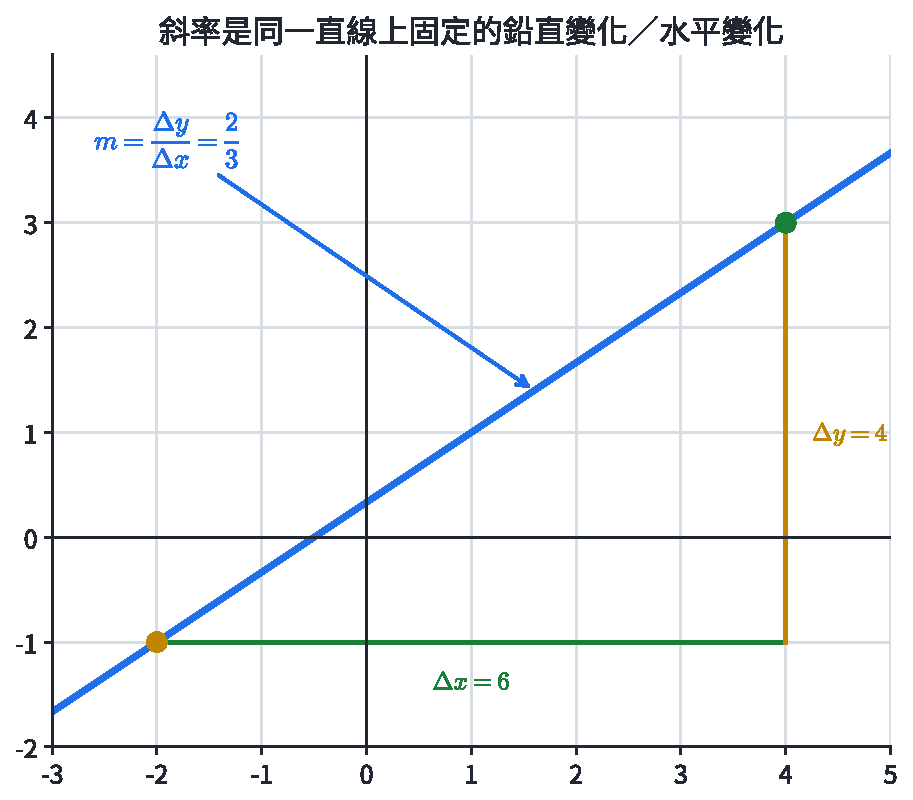
\includegraphics[width=0.94\linewidth,height=\textheight,keepaspectratio,alt={圖 1｜同一直線上任取兩點，斜率三角形的鉛直變化與水平變化維持固定比例。}]{assets/數1-4-斜率三角形.pdf}
\caption{圖 1｜同一直線上任取兩點，斜率三角形的鉛直變化與水平變化維持固定比例。}
\end{figure}

鉛直線 \(x=a\) 的兩點有 \(\Delta x=0\)，斜率不定義；水平線 \(y=b\) 的斜率為 \(0\)。這兩種情形在列方程式時直接使用 \(x=a\) 或 \(y=b\)。

\subsection{1.2 一個點與一個方向決定直線}\label{ux4e00ux500bux9edeux8207ux4e00ux500bux65b9ux5411ux6c7aux5b9aux76f4ux7dda}

斜率為 \(m\) 且通過 \(P(x_1,y_1)\) 的直線上，每一點 \((x,y)\) 都滿足

\[
\frac{y-y_1}{x-x_1}=m.
\]

移項得到點斜式

\[
\boxed{y-y_1=m(x-x_1)}.
\]

由點斜式可整理成幾種常用形式：

\begin{itemize}
\tightlist
\item
  斜截式：\(y=mx+b\)，其中 \(m\) 是斜率，\((0,b)\) 是 \(y\) 軸截點。
\item
  兩點式：\(\dfrac{y-y_1}{y_2-y_1}=\dfrac{x-x_1}{x_2-x_1}\)，適用於兩點的橫坐標、縱坐標皆相異。
\item
  截距式：\(\dfrac{x}{a}+\dfrac{y}{b}=1\)，其中 \((a,0)\)、\((0,b)\) 是兩軸截點，且 \(a,b\ne0\)。
\item
  一般式：\(Ax+By+C=0\)，其中 \(A,B\) 不同時為 \(0\)；它同時容納鉛直線與非鉛直線。
\end{itemize}

\subsection{例 1｜由兩點建立直線方程式}\label{ux4f8b-1ux7531ux5169ux9edeux5efaux7acbux76f4ux7ddaux65b9ux7a0bux5f0f}

求通過 \(P(-2,-1)\)、\(Q(4,3)\) 的直線方程式。

先算斜率：

\[
m=\frac{3-(-1)}{4-(-2)}=\frac46=\frac23.
\]

以 \(P\) 代入點斜式：

\[
y+1=\frac23(x+2).
\]

乘以 \(3\) 並整理：

\[
3y+3=2x+4
\quad\Longrightarrow\quad
\boxed{2x-3y+1=0}.
\]

將 \(P,Q\) 分別代回，左式都等於 \(0\)，所以兩點都在此直線上。

\subsection{例 2｜依資訊選擇方程式形式}\label{ux4f8b-2ux4f9dux8cc7ux8a0aux9078ux64c7ux65b9ux7a0bux5f0fux5f62ux5f0f}

一直線與 \(x\) 軸、\(y\) 軸分別交於 \((6,0)\)、\((0,-3)\)，求其方程式與斜率。

兩個非零截距已知，直接用截距式：

\[
\frac{x}{6}+\frac{y}{-3}=1.
\]

整理得

\[
x-2y=6
\quad\Longrightarrow\quad
y=\frac12x-3.
\]

因此方程式為 \(\boxed{x-2y-6=0}\)，斜率為 \(\boxed{1/2}\)。

\subsubsection{練習 1A}\label{ux7df4ux7fd2-1a}

\begin{enumerate}
\def\labelenumi{\arabic{enumi}.}
\tightlist
\item
  求通過 \((2,-1)\)、\((5,8)\) 的直線方程式。
\item
  求斜率為 \(-2\) 且通過 \((-1,4)\) 的直線方程式。
\item
  一直線的 \(x\) 軸截距為 \(4\)、\(y\) 軸截距為 \(-2\)，求一般式。
\item
  寫出 \(2x+3y-6=0\) 的斜率與兩軸截距。
\item
  分別寫出通過 \((-3,2)\) 的鉛直線，以及通過 \((4,5)\) 的水平線。
\end{enumerate}

\section{2. 平移、平行、垂直與垂足}\label{ux5e73ux79fbux5e73ux884cux5782ux76f4ux8207ux5782ux8db3}

\subsection{2.1 圖形平移反映在坐標替換}\label{ux5716ux5f62ux5e73ux79fbux53cdux6620ux5728ux5750ux6a19ux66ffux63db}

曲線 \(F(x,y)=0\) 向右平移 \(h\)、向上平移 \(k\) 後，新圖形上的點 \((x,y)\) 來自原圖形上的 \((x-h,y-k)\)，因此新方程式是

\[
\boxed{F(x-h,y-k)=0}.
\]

若直線 \(Ax+By+C=0\) 平移後仍是直線，係數 \(A,B\) 保持不變，方向也保持不變；只有常數項改變。

\subsection{2.2 平行與垂直的代數條件}\label{ux5e73ux884cux8207ux5782ux76f4ux7684ux4ee3ux6578ux689dux4ef6}

兩條非鉛直直線斜率分別為 \(m_1,m_2\)：

\[
\boxed{m_1=m_2\iff\text{兩直線平行或重合}},
\]

\[
\boxed{m_1m_2=-1\iff\text{兩直線垂直}}.
\]

第二式可由方向向量推得。斜率 \(m\) 的方向向量可取 \((1,m)\)；兩方向垂直時內積為 \(1+m_1m_2=0\)。

\begin{figure}
\centering
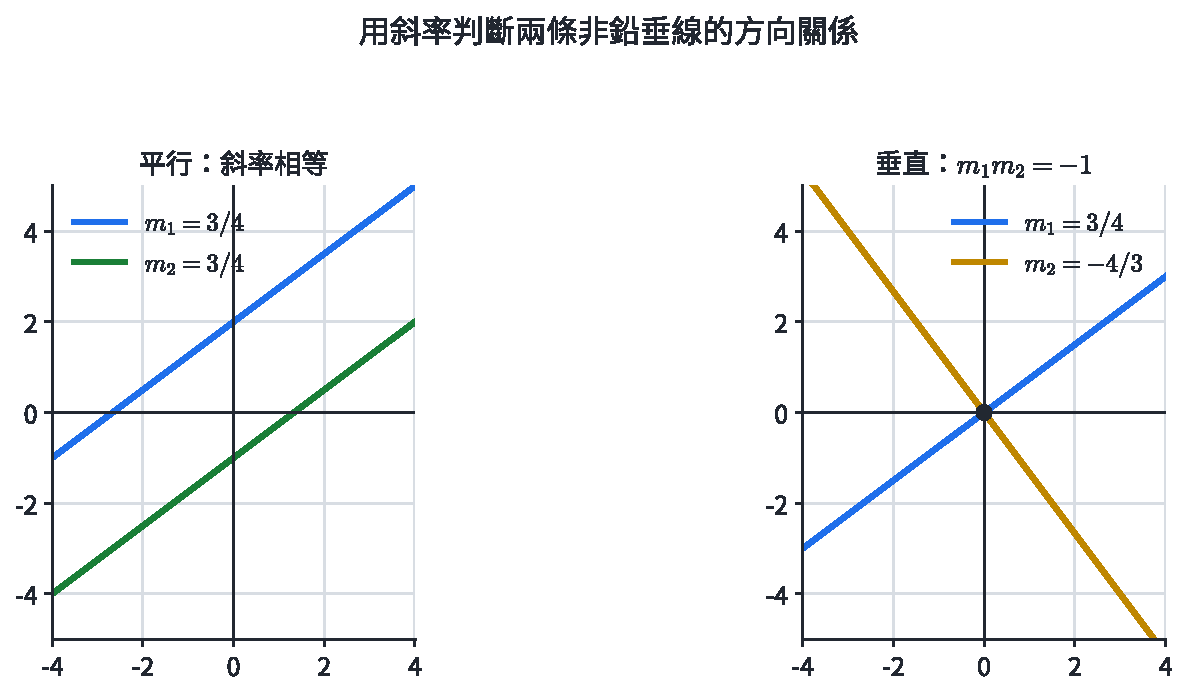
\includegraphics[width=0.94\linewidth,height=\textheight,keepaspectratio,alt={圖 2｜平行直線方向相同；兩條非鉛直、非水平直線垂直時，斜率乘積為 -1。}]{assets/數1-4-平行與垂直.pdf}
\caption{圖 2｜平行直線方向相同；兩條非鉛直、非水平直線垂直時，斜率乘積為 \(-1\)。}
\end{figure}

一般式 \(A_1x+B_1y+C_1=0\)、\(A_2x+B_2y+C_2=0\) 的法向量分別為 \((A_1,B_1)\)、\((A_2,B_2)\)。因此：

\[
A_1B_2-A_2B_1=0\iff\text{方向平行},
\]

\[
A_1A_2+B_1B_2=0\iff\text{兩直線垂直}.
\]

這組係數條件也適用於鉛直線與水平線。

\subsection{例 3｜通過定點的平行線與垂直線}\label{ux4f8b-3ux901aux904eux5b9aux9edeux7684ux5e73ux884cux7ddaux8207ux5782ux76f4ux7dda}

已知 \(L:2x-3y+5=0\)，求通過 \(P(1,4)\) 且分別與 \(L\) 平行、垂直的直線。

\(L\) 的法向量為 \((2,-3)\)。平行線可寫成 \(2x-3y+C=0\)。代入 \(P\)：\(2-12+C=0\)，得 \(C=10\)，所以平行線為

\[
\boxed{2x-3y+10=0}.
\]

與 \(L\) 垂直的直線可取法向量 \((3,2)\)，寫成 \(3x+2y+C=0\)。代入 \(P\) 得 \(3+8+C=0\)，所以

\[
\boxed{3x+2y-11=0}.
\]

\subsection{例 4｜求點到直線的垂足}\label{ux4f8b-4ux6c42ux9edeux5230ux76f4ux7ddaux7684ux5782ux8db3}

求 \(P(1,1)\) 到 \(L:3x-4y+11=0\) 的垂足。

\(L\) 的斜率為 \(3/4\)，垂線斜率為 \(-4/3\)。過 \(P\) 的垂線為

\[
y-1=-\frac43(x-1)
\quad\Longrightarrow\quad
4x+3y-7=0.
\]

聯立

\[
\begin{cases}
3x-4y=-11,\\
4x+3y=7,
\end{cases}
\]

得到 \(\boxed{Q(-1/5,13/5)}\)。由斜率 \(m_{PQ}=-4/3\) 可再確認 \(PQ\perp L\)。

\begin{figure}
\centering
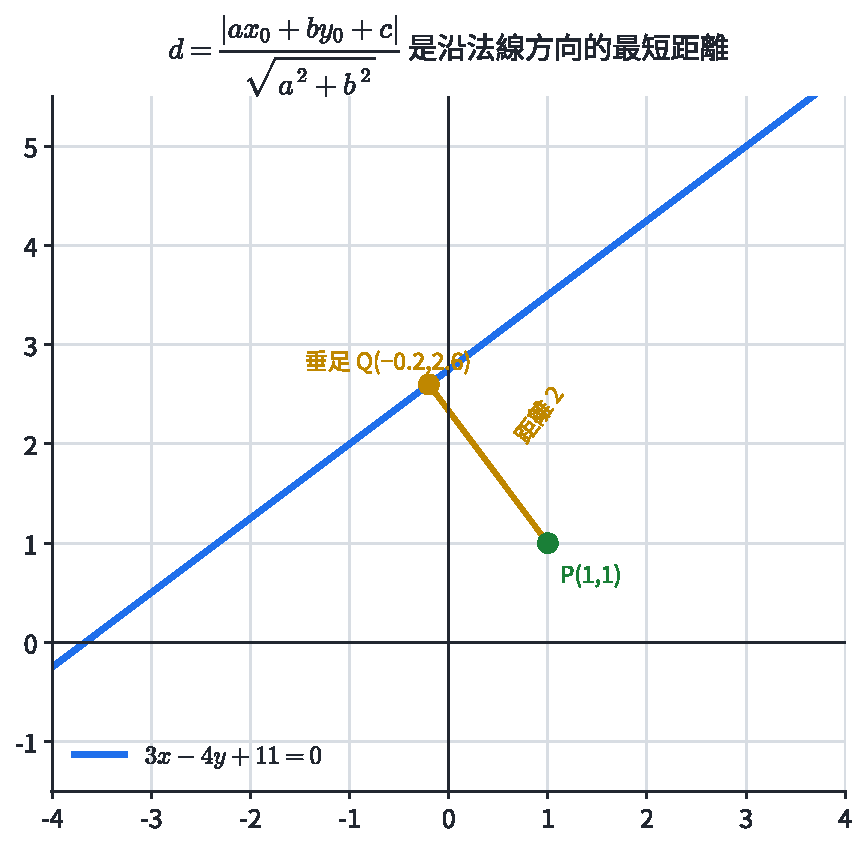
\includegraphics[width=0.88\linewidth,height=\textheight,keepaspectratio,alt={圖 3｜從點 P 沿直線法向量作垂線，與原直線的交點就是垂足。}]{assets/數1-4-點線距離.pdf}
\caption{圖 3｜從點 \(P\) 沿直線法向量作垂線，與原直線的交點就是垂足。}
\end{figure}

\subsubsection{練習 2A}\label{ux7df4ux7fd2-2a}

\begin{enumerate}
\def\labelenumi{\arabic{enumi}.}
\tightlist
\item
  將 \(y=2x-1\) 向右平移 \(3\)、向上平移 \(4\)，求新方程式。
\item
  求通過 \((2,-1)\) 且平行於 \(3x-4y+7=0\) 的直線。
\item
  求通過 \((4,0)\) 且垂直於 \(x+2y-5=0\) 的直線。
\item
  求點 \((1,5)\) 到直線 \(x+y-1=0\) 的垂足。
\item
  若 \(kx+2y-1=0\) 與 \(4x-2y+3=0\) 垂直，求 \(k\)。
\end{enumerate}

\section{3. 聯立方程式與直線距離}\label{ux806fux7acbux65b9ux7a0bux5f0fux8207ux76f4ux7ddaux8dddux96e2}

\subsection{3.1 方程組的解就是幾何交點}\label{ux65b9ux7a0bux7d44ux7684ux89e3ux5c31ux662fux5e7eux4f55ux4ea4ux9ede}

二元一次聯立方程式

\[
\begin{cases}
A_1x+B_1y+C_1=0,\\
A_2x+B_2y+C_2=0
\end{cases}
\]

要求同時落在兩條直線上的點，因此有三種幾何結果：

\begin{itemize}
\tightlist
\item
  兩直線相交：恰有一組解。
\item
  兩直線平行且不同：無解。
\item
  兩方程式描述同一直線：有無限多組解。
\end{itemize}

\begin{figure}
\centering
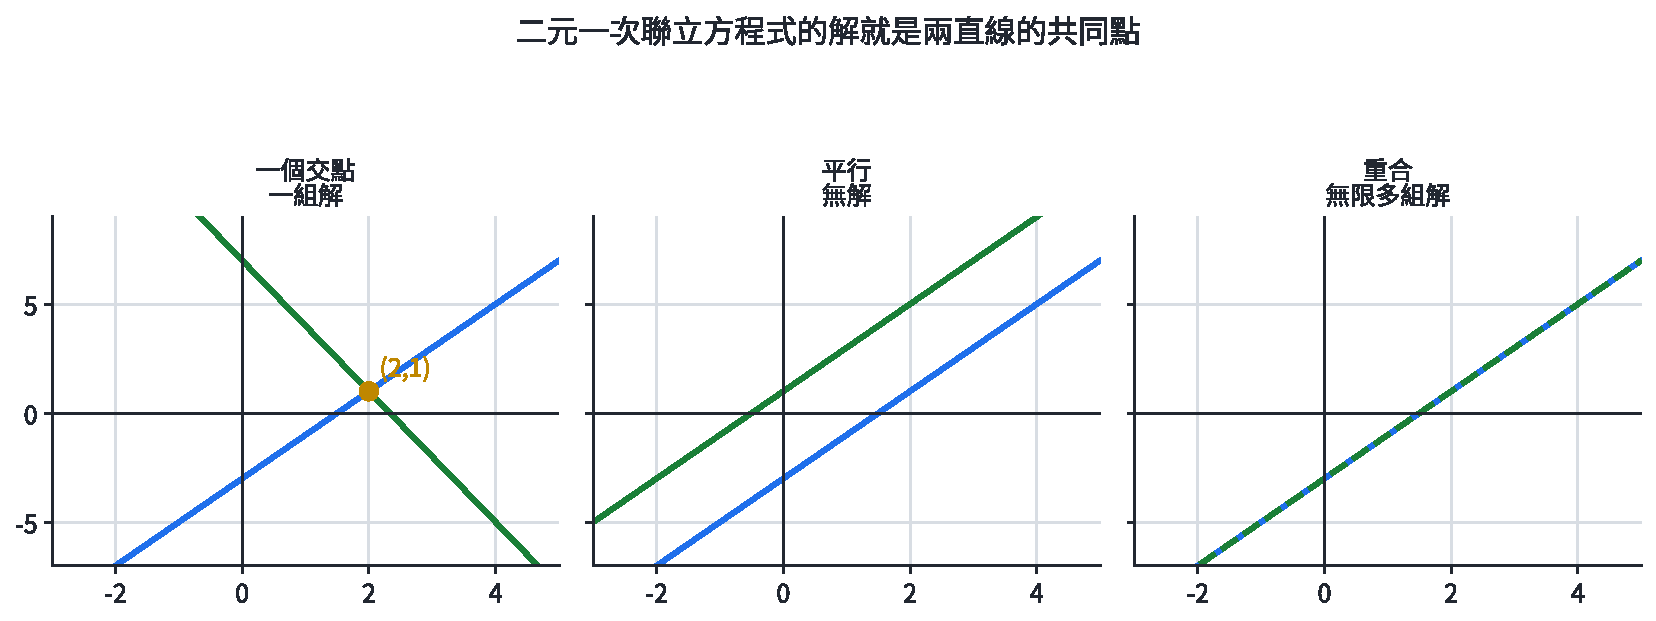
\includegraphics[width=0.98\linewidth,height=\textheight,keepaspectratio,alt={圖 4｜聯立方程式的一組解、無解與無限多組解，分別對應相交、平行與重合。}]{assets/數1-4-聯立方程幾何.pdf}
\caption{圖 4｜聯立方程式的一組解、無解與無限多組解，分別對應相交、平行與重合。}
\end{figure}

若 \(A_1B_2-A_2B_1\ne0\)，兩直線方向不同，必有唯一交點。若此值為 \(0\)，再比較包含常數項的比例，便可區分平行或重合。

\subsection{例 5｜由係數判斷解的個數並求交點}\label{ux4f8b-5ux7531ux4fc2ux6578ux5224ux65b7ux89e3ux7684ux500bux6578ux4e26ux6c42ux4ea4ux9ede}

討論

\[
\begin{cases}
2x-y=3,\\
kx-2y=4
\end{cases}
\]

的解。

兩式係數行列式為

\[
\begin{vmatrix}2&-1\\k&-2\end{vmatrix}=k-4.
\]

當 \(k\ne4\) 時有唯一解。由第一式 \(y=2x-3\)，代入第二式得

\[
(k-4)x=-2,
\]

所以 \(\boxed{x=-2/(k-4)}\)、\(\boxed{y=-4/(k-4)-3}\)。當 \(k=4\) 時，第二式化為 \(2x-y=2\)，與第一式平行且不同，因此無解。

\subsection{3.2 點到直線的距離公式}\label{ux9edeux5230ux76f4ux7ddaux7684ux8dddux96e2ux516cux5f0f}

設 \(P(x_0,y_0)\)，直線 \(L:Ax+By+C=0\)，其中 \((A,B)\ne(0,0)\)。向量 \((A,B)\) 垂直於 \(L\)。從直線上任取 \(Q(x_1,y_1)\)，向量 \(\overrightarrow{QP}\) 在單位法向量上的投影長度就是最短距離：

\[
d=\left|\overrightarrow{QP}\cdot\frac{(A,B)}{\sqrt{A^2+B^2}}\right|.
\]

因為 \(Ax_1+By_1+C=0\)，可化簡為

\[
\boxed{d(P,L)=\frac{|Ax_0+By_0+C|}{\sqrt{A^2+B^2}}}.
\]

絕對值使距離保持非負；分母把法向量正規化，因此同一條直線的方程式乘上任意非零常數，距離仍不變。

\subsection{例 6｜安全距離與平行線間距}\label{ux4f8b-6ux5b89ux5168ux8dddux96e2ux8207ux5e73ux884cux7ddaux9593ux8ddd}

一條管線以 \(3x-4y+20=0\) 表示，控制站位於 \(P(4,1)\)。求站點到管線的最短距離。另求與管線平行、位於原點一側並相距 \(6\) 的直線。

站點到管線的距離為

\[
d=\frac{|3(4)-4(1)+20|}{5}=\frac{28}{5}.
\]

平行線可寫成 \(3x-4y+C=0\)。由 \(|C-20|/5=6\) 得 \(C=50\) 或 \(-10\)。在候選直線上，原管線左式 \(3x-4y+20\) 的值分別為 \(-30\) 與 \(30\)；原點代入原管線左式為 \(20>0\)。因此位於原點一側的平行線是

\[
\boxed{3x-4y-10=0}.
\]

\subsubsection{練習 3A}\label{ux7df4ux7fd2-3a}

\begin{enumerate}
\def\labelenumi{\arabic{enumi}.}
\tightlist
\item
  求 \(x+y=5\) 與 \(2x-y=1\) 的交點。
\item
  判斷 \(2x-3y=1\) 與 \(4x-6y=5\) 所成方程組的解數。
\item
  求點 \((3,-1)\) 到直線 \(4x+3y-6=0\) 的距離。
\item
  求平行線 \(2x-y+3=0\) 與 \(2x-y-7=0\) 的距離。
\item
  求點 \((0,4)\) 到直線 \(3x+4y-12=0\) 的垂足。
\end{enumerate}

\section{4. 二元一次不等式與半平面}\label{ux4e8cux5143ux4e00ux6b21ux4e0dux7b49ux5f0fux8207ux534aux5e73ux9762}

\subsection{4.1 一條直線把平面分成兩側}\label{ux4e00ux689dux76f4ux7ddaux628aux5e73ux9762ux5206ux6210ux5169ux5074}

直線 \(Ax+By+C=0\) 把平面分成 \(Ax+By+C>0\) 與 \(Ax+By+C<0\) 兩個半平面。選一個不在邊界上的測試點代入，即可判定哪一側符合不等式。若是不嚴格不等式 \(\le\) 或 \(\ge\)，邊界直線包含在解集中；若是嚴格不等式 \(<\) 或 \(>\)，邊界不包含在解集中。

兩點 \(P,Q\) 對同一條直線的代入值若同號，兩點位於同側；若異號，兩點位於異側。這是因為沿線段 \(PQ\) 的一次式連續變化，異號時必在中間經過 \(0\)。

\subsection{例 7｜由測試點判定半平面}\label{ux4f8b-7ux7531ux6e2cux8a66ux9edeux5224ux5b9aux534aux5e73ux9762}

畫出 \(2x-y-4\le0\) 的解區域。

邊界為 \(y=2x-4\)。取原點測試，得到 \(-4\le0\)，因此原點所在側是解區域，邊界也包含在內。等價地，原不等式可整理成

\[
\boxed{y\ge2x-4}.
\]

\subsection{4.2 多個限制取交集}\label{ux591aux500bux9650ux5236ux53d6ux4ea4ux96c6}

聯立二元一次不等式的解，是各半平面的交集。邊界直線的交點與坐標軸截點常形成可行區域的頂點；把每個頂點代回全部不等式，可以檢查是否真的屬於交集。

\subsection{例 8｜求聯立不等式的可行區域頂點}\label{ux4f8b-8ux6c42ux806fux7acbux4e0dux7b49ux5f0fux7684ux53efux884cux5340ux57dfux9802ux9ede}

求

\[
\begin{cases}
x\ge0,\\
y\ge0,\\
2x+y\le4,\\
x+3y\le6
\end{cases}
\]

的可行區域頂點。

兩條斜邊聯立得 \((x,y)=(6/5,8/5)\)。坐標軸上同時符合全部限制的端點是 \((2,0)\) 與 \((0,2)\)，再加上原點。因此頂點為

\[
\boxed{(0,0),\ (2,0),\ (6/5,8/5),\ (0,2)}.
\]

\begin{figure}
\centering
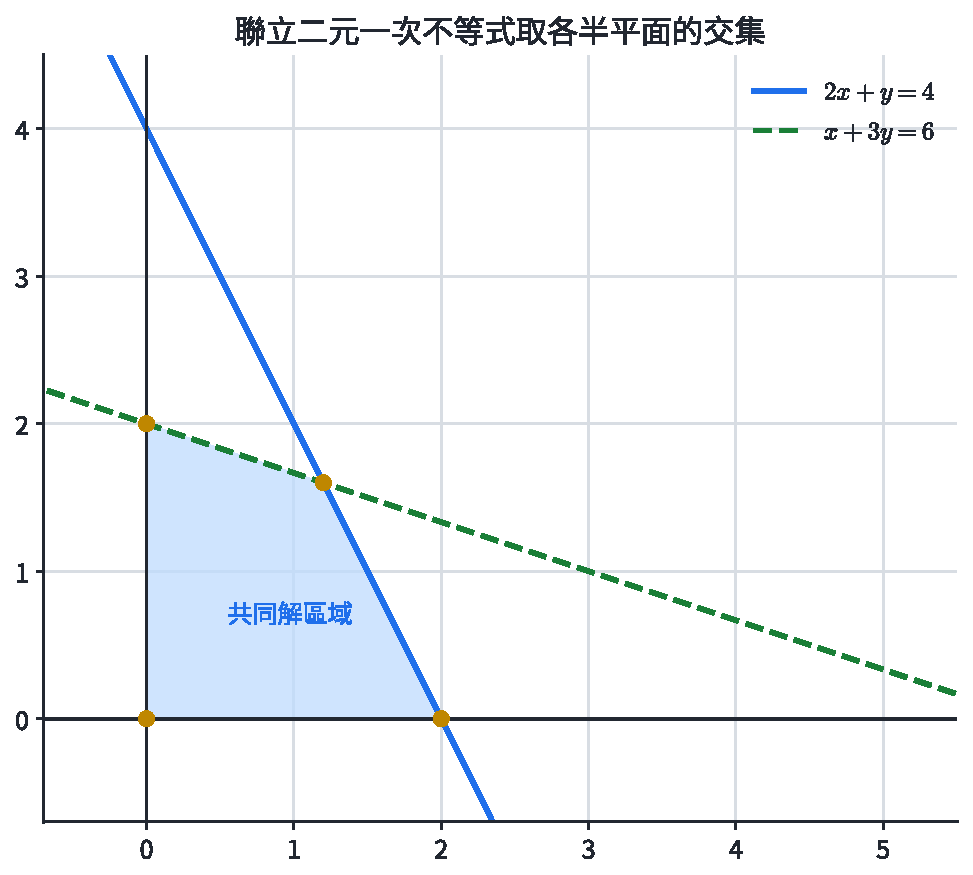
\includegraphics[width=0.9\linewidth,height=\textheight,keepaspectratio,alt={圖 5｜每個不等式給出一個半平面；共同解是所有半平面的交集。}]{assets/數1-4-半平面.pdf}
\caption{圖 5｜每個不等式給出一個半平面；共同解是所有半平面的交集。}
\end{figure}

\subsubsection{練習 4A}\label{ux7df4ux7fd2-4a}

\begin{enumerate}
\def\labelenumi{\arabic{enumi}.}
\tightlist
\item
  說明 \(2x+y\le4\) 的邊界是否包含在解集中，並判斷原點所在側是否為解區域。
\item
  求 \(x\ge0,y\ge0,2x+y\le4,x+3y\le6\) 的所有頂點。
\item
  判斷 \(A(1,1)\)、\(B(3,4)\) 位於直線 \(x-2y+3=0\) 的同側或異側。
\item
  將 \(y>2x-1\) 寫成一般式不等式，並說明原點是否在解區域。
\item
  求 \(x\ge0,y\ge0,x+y\le5,2x+y\ge4\) 的所有頂點。
\end{enumerate}

\section{5. 圓的方程式與點的位置}\label{ux5713ux7684ux65b9ux7a0bux5f0fux8207ux9edeux7684ux4f4dux7f6e}

\subsection{5.1 圓的定義直接產生標準式}\label{ux5713ux7684ux5b9aux7fa9ux76f4ux63a5ux7522ux751fux6a19ux6e96ux5f0f}

圓是平面上到固定點 \(C(h,k)\) 的距離都等於正數 \(r\) 的點集。由距離公式，點 \(P(x,y)\) 在圓上等價於

\[
\sqrt{(x-h)^2+(y-k)^2}=r.
\]

兩邊平方得到標準式

\[
\boxed{(x-h)^2+(y-k)^2=r^2},\qquad r>0.
\]

\begin{figure}
\centering
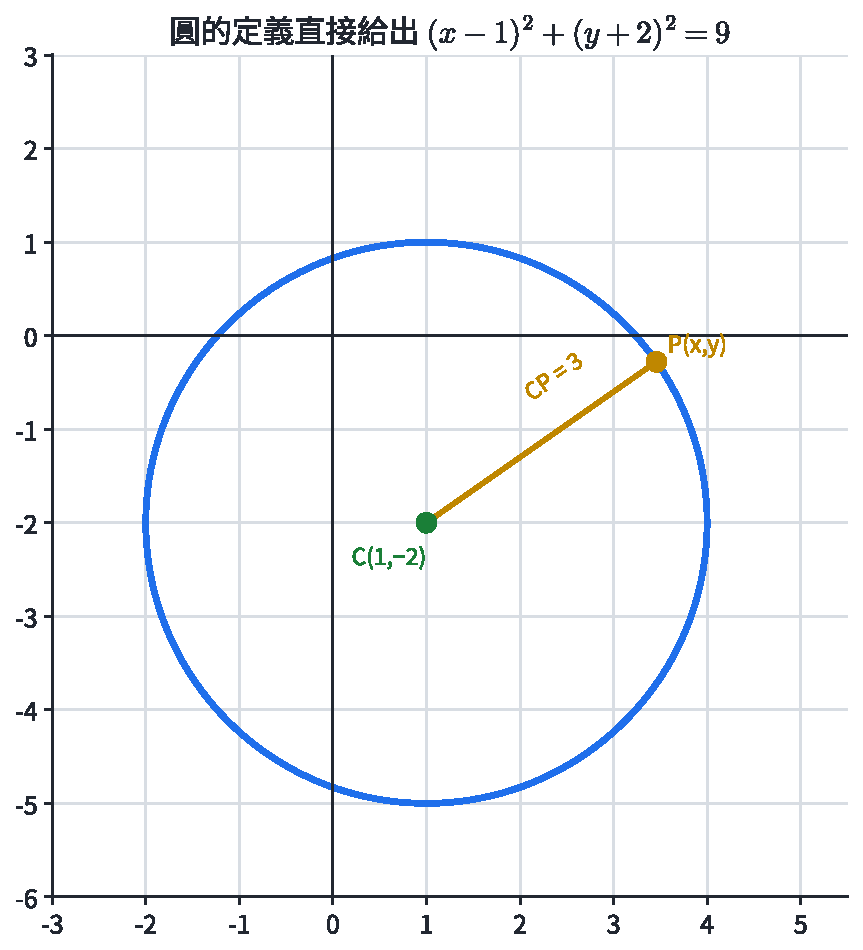
\includegraphics[width=0.86\linewidth,height=\textheight,keepaspectratio,alt={圖 6｜圓上每一點到圓心的距離都等於半徑；方程式就是距離定義的平方。}]{assets/數1-4-圓方程式.pdf}
\caption{圖 6｜圓上每一點到圓心的距離都等於半徑；方程式就是距離定義的平方。}
\end{figure}

若已知圓的直徑端點 \(A,B\)，圓心是線段中點，半徑是 \(AB/2\)。這比直接設一般式的三個未知係數更有效率。

\subsection{5.2 一般式與存在條件}\label{ux4e00ux822cux5f0fux8207ux5b58ux5728ux689dux4ef6}

展開標準式可得

\[
x^2+y^2+Dx+Ey+F=0.
\]

配方後成為

\[
\left(x+\frac D2\right)^2+
\left(y+\frac E2\right)^2
=\frac{D^2+E^2}{4}-F.
\]

因此圓心與半徑平方為

\[
\boxed{C\left(-\frac D2,-\frac E2\right)},\qquad
\boxed{r^2=\frac{D^2+E^2}{4}-F}.
\]

\(r^2>0\) 時是圓；\(r^2=0\) 時只剩圓心一點；\(r^2<0\) 時沒有實數點。

\subsection{例 9｜由三點決定圓}\label{ux4f8b-9ux7531ux4e09ux9edeux6c7aux5b9aux5713}

求通過 \(A(0,0)\)、\(B(4,0)\)、\(C(0,6)\) 的圓。

設一般式為

\[
x^2+y^2+Dx+Ey+F=0.
\]

代入 \(A\) 得 \(F=0\)；代入 \(B\) 得 \(16+4D=0\)，所以 \(D=-4\)；代入 \(C\) 得 \(36+6E=0\)，所以 \(E=-6\)。圓為

\[
x^2+y^2-4x-6y=0.
\]

配方得到

\[
\boxed{(x-2)^2+(y-3)^2=13}.
\]

圓心 \((2,3)\) 正是直角三角形 \(ABC\) 斜邊 \(BC\) 的中點。

\subsection{例 10｜參數何時代表真正的圓}\label{ux4f8b-10ux53c3ux6578ux4f55ux6642ux4ee3ux8868ux771fux6b63ux7684ux5713}

討論

\[
x^2+y^2-2ax+4y+2a=0
\]

在不同 \(a\) 下的圖形。

配方得

\[
(x-a)^2+(y+2)^2=a^2-2a+4=(a-1)^2+3.
\]

右式對所有實數 \(a\) 都大於 \(0\)，因此每一個實數 \(a\) 都給出真正的圓。圓心與半徑為

\[
\boxed{(a,-2)},\qquad
\boxed{\sqrt{(a-1)^2+3}}.
\]

\subsection{5.3 點在圓內、圓上或圓外}\label{ux9edeux5728ux5713ux5167ux5713ux4e0aux6216ux5713ux5916}

對圓 \((x-h)^2+(y-k)^2=r^2\) 與點 \(P(x_0,y_0)\)，比較

\[
PC^2=(x_0-h)^2+(y_0-k)^2
\]

和 \(r^2\)：小於時在圓內，等於時在圓上，大於時在圓外。使用平方距離即可完成判斷，無須先開根號。

\subsubsection{練習 5A}\label{ux7df4ux7fd2-5a}

\begin{enumerate}
\def\labelenumi{\arabic{enumi}.}
\tightlist
\item
  寫出圓心 \((-2,3)\)、半徑 \(4\) 的圓方程式。
\item
  將 \(x^2+y^2-6x+4y-3=0\) 化為標準式，並求圓心、半徑。
\item
  判斷 \(x^2+y^2+2ax-4y+a=0\) 對哪些實數 \(a\) 表示真正的圓。
\item
  判斷點 \((5,1)\) 在圓 \((x-1)^2+(y-1)^2=9\) 的內部、圓上或外部。
\item
  圓的直徑端點為 \((-1,2)\)、\((5,-4)\)，求圓方程式。
\end{enumerate}

\section{6. 圓與直線的位置關係}\label{ux5713ux8207ux76f4ux7ddaux7684ux4f4dux7f6eux95dcux4fc2}

\subsection{6.1 比較圓心到直線的距離與半徑}\label{ux6bd4ux8f03ux5713ux5fc3ux5230ux76f4ux7ddaux7684ux8dddux96e2ux8207ux534aux5f91}

設圓心到直線的距離為 \(d\)、圓半徑為 \(r\)。沿圓心到直線的垂線觀察：

\[
\boxed{
\begin{array}{ccl}
d<r&\Longrightarrow&\text{兩個交點},\\
d=r&\Longrightarrow&\text{一個交點，直線為切線},\\
d>r&\Longrightarrow&\text{沒有交點}.
\end{array}}
\]

\begin{figure}
\centering
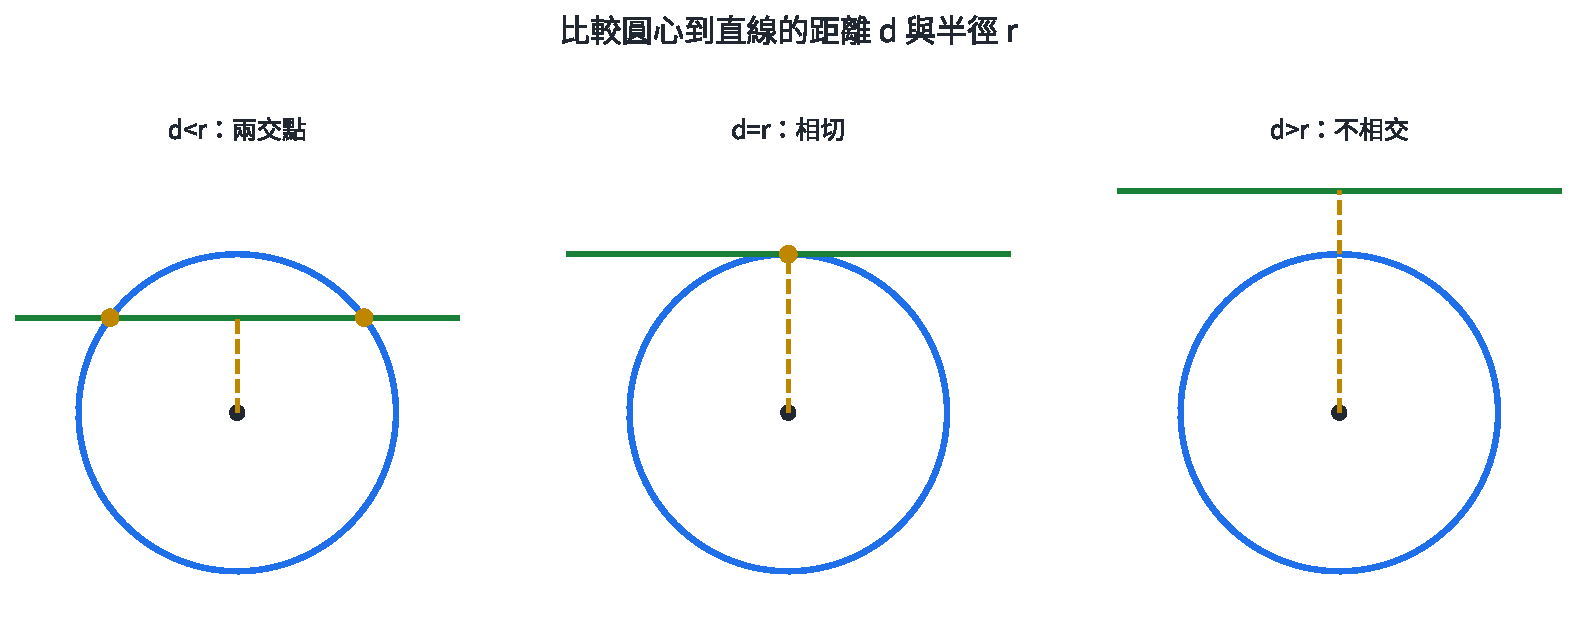
\includegraphics[width=0.98\linewidth,height=\textheight,keepaspectratio,alt={圖 7｜圓心到直線的最短距離與半徑，直接決定相交、相切或不相交。}]{assets/數1-4-圓與直線位置.pdf}
\caption{圖 7｜圓心到直線的最短距離與半徑，直接決定相交、相切或不相交。}
\end{figure}

這個方法只需一次距離計算，適合判斷交點個數。若題目還要求交點坐標，則把直線方程式代入圓，解所得的一元二次方程式。

\subsection{例 11｜以距離判斷位置關係}\label{ux4f8b-11ux4ee5ux8dddux96e2ux5224ux65b7ux4f4dux7f6eux95dcux4fc2}

判斷直線 \(3x-4y+1=0\) 與圓

\[
(x-2)^2+(y+1)^2=9
\]

的位置關係。

圓心為 \((2,-1)\)，半徑 \(r=3\)。圓心到直線的距離為

\[
d=\frac{|3(2)-4(-1)+1|}{5}=\frac{11}{5}.
\]

因為 \(11/5<3\)，所以直線穿過圓，有 \(\boxed{2\text{ 個交點}}\)。

\subsection{例 12｜求直線截圓所得的交點}\label{ux4f8b-12ux6c42ux76f4ux7ddaux622aux5713ux6240ux5f97ux7684ux4ea4ux9ede}

求直線 \(y=x+1\) 與圓 \(x^2+y^2=5\) 的交點。

代入 \(y=x+1\)：

\[
x^2+(x+1)^2=5
\quad\Longrightarrow\quad
x^2+x-2=0.
\]

因式分解為 \((x-1)(x+2)=0\)，所以 \(x=1\) 或 \(-2\)。由 \(y=x+1\) 得

\[
\boxed{(1,2),\ (-2,-1)}.
\]

兩點代回圓方程式都得到 \(5\)，也都滿足直線方程式。

\subsubsection{練習 6A}\label{ux7df4ux7fd2-6a}

\begin{enumerate}
\def\labelenumi{\arabic{enumi}.}
\tightlist
\item
  求圓 \(x^2+y^2=25\) 與直線 \(y=3\) 的交點。
\item
  判斷 \(3x+4y-20=0\) 與 \(x^2+y^2=16\) 的位置關係。
\item
  判斷直線 \(x=6\) 與圓 \((x-2)^2+(y+1)^2=9\) 的位置關係。
\item
  討論水平線 \(y=k\) 與單位圓 \(x^2+y^2=1\) 的交點個數。
\item
  求 \(x^2+y^2=13\) 與 \(x+y=5\) 的交點。
\end{enumerate}

\section{7. 圓的切線}\label{ux5713ux7684ux5207ux7dda}

\subsection{7.1 切點半徑是切線的法向量}\label{ux5207ux9edeux534aux5f91ux662fux5207ux7ddaux7684ux6cd5ux5411ux91cf}

若直線在 \(T(x_1,y_1)\) 與圓相切，圓心 \(C(h,k)\) 到直線的最短線段就是 \(CT\)，因此 \(CT\) 垂直切線。向量 \(\overrightarrow{CT}=(x_1-h,y_1-k)\) 可直接作為切線的法向量。切線方程式為

\[
\boxed{(x_1-h)(x-x_1)+(y_1-k)(y-y_1)=0}.
\]

這個式子也適用於鉛直切線，不需要另外計算斜率。

\begin{figure}
\centering
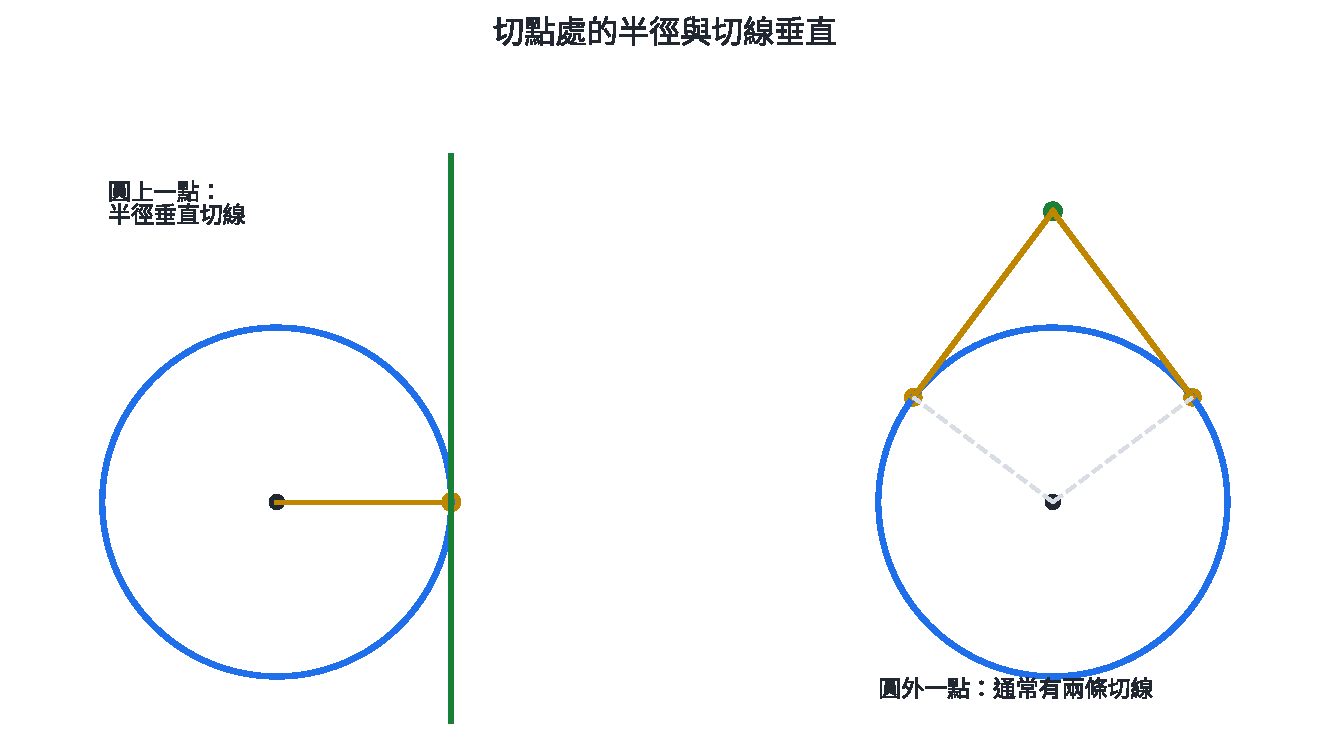
\includegraphics[width=0.98\linewidth,height=\textheight,keepaspectratio,alt={圖 8｜已知切點時用半徑作法向量；圓外一點通常可連出兩條切線。}]{assets/數1-4-圓的切線.pdf}
\caption{圖 8｜已知切點時用半徑作法向量；圓外一點通常可連出兩條切線。}
\end{figure}

\subsection{例 13｜已知切點求切線}\label{ux4f8b-13ux5df2ux77e5ux5207ux9edeux6c42ux5207ux7dda}

求圓 \((x-2)^2+(y+1)^2=25\) 在 \(T(5,3)\) 的切線。

圓心 \(C(2,-1)\)，所以 \(\overrightarrow{CT}=(3,4)\)。以 \((3,4)\) 為切線法向量：

\[
3(x-5)+4(y-3)=0.
\]

整理得

\[
\boxed{3x+4y-27=0}.
\]

圓心到此直線的距離為 \(|3(2)+4(-1)-27|/5=5\)，等於半徑。

\subsection{7.2 已知斜率或圓外點求切線}\label{ux5df2ux77e5ux659cux7387ux6216ux5713ux5916ux9edeux6c42ux5207ux7dda}

斜率為 \(m\) 的直線可寫成 \(y=mx+b\)，即 \(mx-y+b=0\)。它與圓心 \((h,k)\)、半徑 \(r\) 的圓相切，等價於

\[
\boxed{\frac{|mh-k+b|}{\sqrt{m^2+1}}=r}.
\]

若切線還通過已知圓外點，先用該點把 \(b\) 寫成 \(m\) 的式子，再解距離條件。圓外點通常得到兩個斜率；若其中一條切線鉛直，斜截式不會包含它，此時需另檢查 \(x=\text{常數}\)。

\subsection{例 14｜由圓外點作兩條切線}\label{ux4f8b-14ux7531ux5713ux5916ux9edeux4f5cux5169ux689dux5207ux7dda}

由 \(P(0,5)\) 向圓 \(x^2+y^2=9\) 作切線，求切線方程式。

通過 \(P\) 的非鉛直直線寫成 \(y=mx+5\)。相切條件為

\[
\frac5{\sqrt{m^2+1}}=3.
\]

平方後得到 \(25=9m^2+9\)，所以 \(m=\pm4/3\)。兩條切線為

\[
\boxed{y=\frac43x+5},\qquad
\boxed{y=-\frac43x+5}.
\]

\(P\) 的橫坐標為 \(0\)，鉛直線 \(x=0\) 通過圓心並穿過圓，因此不形成遺漏的鉛直切線。

\subsubsection{練習 7A}\label{ux7df4ux7fd2-7a}

\begin{enumerate}
\def\labelenumi{\arabic{enumi}.}
\tightlist
\item
  求圓 \(x^2+y^2=25\) 在 \((3,4)\) 的切線。
\item
  求圓 \((x-1)^2+(y+2)^2=9\) 在 \((4,-2)\) 的切線。
\item
  求斜率為 \(2\) 且與 \(x^2+y^2=5\) 相切的所有直線。
\item
  由 \((0,5)\) 向 \(x^2+y^2=9\) 作切線，求兩條切線。
\item
  直線 \(x=t\) 與圓 \(x^2+y^2=4\) 相切，求 \(t\)。
\end{enumerate}

\section{8. 分節練習完整解析}\label{ux5206ux7bc0ux7df4ux7fd2ux5b8cux6574ux89e3ux6790}

\subsection{練習 1A}\label{ux7df4ux7fd2-1a-1}

\begin{enumerate}
\def\labelenumi{\arabic{enumi}.}
\tightlist
\item
  \(m=(8+1)/(5-2)=3\)，所以 \(y+1=3(x-2)\)，即 \(\boxed{3x-y-7=0}\)。
\item
  \(y-4=-2(x+1)\)，所以 \(\boxed{y=-2x+2}\)。
\item
  \(x/4+y/(-2)=1\)，整理得 \(\boxed{x-2y-4=0}\)。
\item
  \(y=-\frac23x+2\)，所以斜率為 \(\boxed{-2/3}\)，\(x\) 軸截距為 \(\boxed3\)，\(y\) 軸截距為 \(\boxed2\)。
\item
  鉛直線為 \(\boxed{x=-3}\)；水平線為 \(\boxed{y=5}\)。
\end{enumerate}

\subsection{練習 2A}\label{ux7df4ux7fd2-2a-1}

\begin{enumerate}
\def\labelenumi{\arabic{enumi}.}
\tightlist
\item
  新圖形滿足 \(y-4=2(x-3)-1\)，所以 \(\boxed{y=2x-3}\)。
\item
  設 \(3x-4y+C=0\)，代入 \((2,-1)\) 得 \(6+4+C=0\)，所以 \(\boxed{3x-4y-10=0}\)。
\item
  原直線斜率為 \(-1/2\)，垂線斜率為 \(2\)。\(y=2(x-4)\)，所以 \(\boxed{y=2x-8}\)。
\item
  原直線斜率 \(-1\)，垂線斜率 \(1\)。過 \((1,5)\) 的垂線為 \(y=x+4\)，與 \(x+y=1\) 聯立得垂足 \(\boxed{(-3/2,5/2)}\)。
\item
  兩直線法向量為 \((k,2)\)、\((4,-2)\)。直線垂直時法向量也垂直，故 \(4k-4=0\)，\(\boxed{k=1}\)。
\end{enumerate}

\subsection{練習 3A}\label{ux7df4ux7fd2-3a-1}

\begin{enumerate}
\def\labelenumi{\arabic{enumi}.}
\tightlist
\item
  兩式相加得 \(3x=6\)，所以 \(x=2,y=3\)，交點為 \(\boxed{(2,3)}\)。
\item
  第二式左側是第一式左側的 \(2\) 倍，但右側不是 \(2\)，兩直線平行且不同，方程組 \(\boxed{\text{無解}}\)。
\item
  \(d=|4(3)+3(-1)-6|/5=\boxed{3/5}\)。
\item
  兩式已使用相同的 \(x,y\) 係數，距離為 \(|3-(-7)|/\sqrt5=\boxed{2\sqrt5}\)。
\item
  設 \(s=3(0)+4(4)-12=4\)。沿法向量移至直線：
  \[
  Q=(0,4)-\frac4{25}(3,4)=\boxed{\left(-\frac{12}{25},\frac{84}{25}\right)}.
  \]
  代入直線左式得 \(0\)，確認 \(Q\) 在直線上。
\end{enumerate}

\subsection{練習 4A}\label{ux7df4ux7fd2-4a-1}

\begin{enumerate}
\def\labelenumi{\arabic{enumi}.}
\tightlist
\item
  符號為 \(\le\)，所以邊界包含在解集中。原點代入得 \(0\le4\)，因此原點所在側是解區域。
\item
  兩斜線交點為 \((6/5,8/5)\)；連同坐標軸邊界，頂點為 \(\boxed{(0,0),(2,0),(6/5,8/5),(0,2)}\)。
\item
  代入一次式 \(x-2y+3\)：\(A\) 得 \(2>0\)，\(B\) 得 \(-2<0\)，所以兩點在 \(\boxed{\text{異側}}\)。
\item
  一般式為 \(\boxed{2x-y-1<0}\)。原點代入得 \(-1<0\)，所以原點在解區域。
\item
  邊界交點與坐標軸端點依序為 \(\boxed{(0,4),(0,5),(5,0),(2,0)}\)；每一點都符合四個限制。
\end{enumerate}

\subsection{練習 5A}\label{ux7df4ux7fd2-5a-1}

\begin{enumerate}
\def\labelenumi{\arabic{enumi}.}
\tightlist
\item
  \(\boxed{(x+2)^2+(y-3)^2=16}\)。
\item
  配方得 \(\boxed{(x-3)^2+(y+2)^2=16}\)，圓心 \(\boxed{(3,-2)}\)，半徑 \(\boxed4\)。
\item
  配方後半徑平方為 \(a^2-a+4=(a-1/2)^2+15/4>0\)，所以 \(\boxed{a\in\mathbb R}\) 都表示真正的圓。
\item
  到圓心 \((1,1)\) 的距離平方為 \(16>9\)，所以點在 \(\boxed{\text{圓外}}\)。
\item
  中點為 \((2,-1)\)，直徑平方為 \(72\)，所以半徑平方為 \(18\)。圓為 \(\boxed{(x-2)^2+(y+1)^2=18}\)。
\end{enumerate}

\subsection{練習 6A}\label{ux7df4ux7fd2-6a-1}

\begin{enumerate}
\def\labelenumi{\arabic{enumi}.}
\tightlist
\item
  \(x^2+3^2=25\)，所以 \(x=\pm4\)，交點為 \(\boxed{(4,3),(-4,3)}\)。
\item
  圓心到直線距離為 \(20/5=4\)，等於半徑，故 \(\boxed{\text{相切}}\)。
\item
  圓心 \((2,-1)\) 到 \(x=6\) 的距離為 \(4>3\)，故 \(\boxed{\text{不相交}}\)。
\item
  圓心到 \(y=k\) 的距離為 \(|k|\)。\(|k|<1\) 有兩點；\(|k|=1\) 相切；\(|k|>1\) 無交點。
\item
  令 \(y=5-x\)，代入圓得 \(x^2-5x+6=0\)，所以交點為 \(\boxed{(2,3),(3,2)}\)。
\end{enumerate}

\subsection{練習 7A}\label{ux7df4ux7fd2-7a-1}

\begin{enumerate}
\def\labelenumi{\arabic{enumi}.}
\tightlist
\item
  半徑向量為 \((3,4)\)，故切線為 \(\boxed{3x+4y=25}\)。
\item
  切點半徑水平，切線鉛直，所以 \(\boxed{x=4}\)。
\item
  設 \(y=2x+b\)。圓心到直線距離為 \(|b|/\sqrt5\)，令其等於 \(\sqrt5\) 得 \(|b|=5\)。兩線為 \(\boxed{y=2x+5}\)、\(\boxed{y=2x-5}\)。
\item
  依相切距離條件得 \(m=\pm4/3\)，所以 \(\boxed{y=\frac43x+5}\)、\(\boxed{y=-\frac43x+5}\)。
\item
  圓心到 \(x=t\) 的距離為 \(|t|\)，令 \(|t|=2\)，得 \(\boxed{t=\pm2}\)。
\end{enumerate}

\section{9. 章末代表題}\label{ux7ae0ux672bux4ee3ux8868ux984c}

\subsection{基礎層}\label{ux57faux790eux5c64}

\begin{enumerate}
\def\labelenumi{\arabic{enumi}.}
\tightlist
\item
  求通過 \((-2,3)\)、\((4,-1)\) 的直線一般式。
\item
  求通過 \((6,2)\) 且垂直於 \(3x-y+4=0\) 的直線。
\item
  將 \(2x-y+1=0\) 向左平移 \(2\)、向下平移 \(3\)，求新方程式。
\item
  求 \(2x+y=7\) 與 \(x-y=2\) 的交點。
\item
  求點 \((2,-3)\) 到 \(x-2y+4=0\) 的距離。
\item
  求平行線 \(3x+4y-8=0\) 與 \(3x+4y+7=0\) 的距離。
\item
  描述不等式 \(x-2y+4>0\) 的解區域，並說明邊界是否包含。
\item
  求 \(x\ge0,y\ge0,x+y\le6,2x+y\ge4\) 的可行區域頂點。
\end{enumerate}

\subsection{進階層}\label{ux9032ux968eux5c64}

\begin{enumerate}
\def\labelenumi{\arabic{enumi}.}
\setcounter{enumi}{8}
\tightlist
\item
  求圓心 \((-3,2)\) 且通過 \((1,5)\) 的圓方程式。
\item
  將 \(x^2+y^2+4x-6y-12=0\) 化為標準式。
\item
  判斷 \((4,1)\) 與圓 \((x-1)^2+(y+1)^2=13\) 的位置關係。
\item
  求 \(y=x+1\) 與 \(x^2+y^2=5\) 的交點。
\end{enumerate}

\subsection{跨節整合}\label{ux8de8ux7bc0ux6574ux5408}

\begin{enumerate}
\def\labelenumi{\arabic{enumi}.}
\setcounter{enumi}{12}
\tightlist
\item
  圓 \((x-2)^2+(y-1)^2=25\) 上有一點 \(T(5,5)\)。求切線，並以圓心到直線距離檢查相切。
\item
  求斜率為 \(-1\) 且與圓 \(x^2+y^2=2\) 相切的所有直線。
\item
  圓形安全區中心為 \(P(2,1)\)、半徑為 \(3\)，道路中心線為 \(3x-4y+12=0\)。判斷道路是否進入安全區，並給出最短距離。
\item
  由觀測點 \(A(0,13)\) 向圓 \(x^2+y^2=25\) 作切線。求兩條切線方程式與兩個切點坐標。
\end{enumerate}

\section{10. 章末代表題完整詳解}\label{ux7ae0ux672bux4ee3ux8868ux984cux5b8cux6574ux8a73ux89e3}

\begin{enumerate}
\def\labelenumi{\arabic{enumi}.}
\tightlist
\item
  斜率為 \((-1-3)/(4+2)=-2/3\)。由 \(y-3=-\frac23(x+2)\)，得 \(\boxed{2x+3y-5=0}\)。
\item
  原直線斜率為 \(3\)，垂線斜率為 \(-1/3\)。\(y-2=-\frac13(x-6)\)，所以 \(\boxed{x+3y-12=0}\)。
\item
  平移向量為 \((-2,-3)\)，新圖形滿足 \(2(x+2)-(y+3)+1=0\)，故 \(\boxed{2x-y+2=0}\)。
\item
  兩式相加得 \(3x=9\)，所以交點為 \(\boxed{(3,1)}\)。
\item
  距離為
  \[
  \frac{|2-2(-3)+4|}{\sqrt{1^2+(-2)^2}}
  =\boxed{\frac{12}{\sqrt5}}.
  \]
\item
  兩式法向量相同，距離為 \(|(-8)-7|/5=\boxed3\)。
\item
  整理成 \(y<(x+4)/2\)。原點代入原式得 \(4>0\)，所以原點所在側是解區域；嚴格不等式的邊界 \(x-2y+4=0\) 不包含在內。
\item
  在 \(x\) 軸上，\(2\le x\le6\)；在 \(y\) 軸上，\(4\le y\le6\)。四個頂點為 \(\boxed{(2,0),(6,0),(0,6),(0,4)}\)。
\item
  半徑平方為 \((1+3)^2+(5-2)^2=25\)，所以 \(\boxed{(x+3)^2+(y-2)^2=25}\)。
\item
  配方得
  \[
  (x+2)^2+(y-3)^2=4+9+12=25.
  \]
  所以標準式為 \(\boxed{(x+2)^2+(y-3)^2=25}\)。
\item
  點到圓心 \((1,-1)\) 的距離平方為 \((4-1)^2+(1+1)^2=13\)，等於半徑平方，因此點 \(\boxed{\text{在圓上}}\)。
\item
  代入 \(y=x+1\)：\(x^2+(x+1)^2=5\)，得 \((x-1)(x+2)=0\)。交點為 \(\boxed{(1,2),(-2,-1)}\)。
\item
  圓心 \(C(2,1)\)，\(\overrightarrow{CT}=(3,4)\)，所以切線為
  \[
  3(x-5)+4(y-5)=0
  \quad\Longrightarrow\quad
  \boxed{3x+4y-35=0}.
  \]
  圓心到切線距離為 \(|6+4-35|/5=5\)，等於半徑，確認相切。
\item
  設直線為 \(y=-x+b\)，即 \(x+y-b=0\)。圓心到直線距離為 \(|b|/\sqrt2\)；令其等於半徑 \(\sqrt2\)，得 \(|b|=2\)。兩切線為 \(\boxed{y=-x+2}\)、\(\boxed{y=-x-2}\)。
\item
  圓心到道路距離為
  \[
  d=\frac{|3(2)-4(1)+12|}{5}=\frac{14}{5}=2.8.
  \]
  因為 \(d<3\)，道路有一段位於圓形安全區內，故 \(\boxed{\text{道路進入安全區}}\)。
\item
  通過 \(A\) 的非鉛直直線寫成 \(y=mx+13\)。相切條件為
  \[
  \frac{13}{\sqrt{m^2+1}}=5
  \quad\Longrightarrow\quad
  m=\pm\frac{12}{5}.
  \]
  兩切線為
  \[
  \boxed{12x-5y+65=0},\qquad
  \boxed{-12x-5y+65=0}.
  \]
  切點是圓心到各切線的垂足。對第一條線，
  \[
  T_1=-\frac{65}{12^2+(-5)^2}(12,-5)
  =\left(-\frac{60}{13},\frac{25}{13}\right).
  \]
  由對稱性，另一切點為
  \[
  \boxed{T_2=\left(\frac{60}{13},\frac{25}{13}\right)}.
  \]
  兩點的距離平方都是 \(25\)，並分別滿足對應切線方程式。
\end{enumerate}

\section{11. 核心整理}\label{ux6838ux5fc3ux6574ux7406}

\begin{itemize}
\tightlist
\item
  斜率 \(m=\Delta y/\Delta x\) 描述直線的固定方向；鉛直線直接寫成 \(x=a\)。
\item
  點斜式 \(y-y_1=m(x-x_1)\) 由一點與一個方向建立直線；一般式 \(Ax+By+C=0\) 同時容納所有直線。
\item
  平行可比較斜率或係數比例；垂直可用斜率乘積 \(-1\) 或法向量內積為 \(0\)。
\item
  聯立兩個一次方程式就是找兩條直線的共同點；相交、平行、重合分別對應一組解、無解、無限多組解。
\item
  點到直線距離為 \(|Ax_0+By_0+C|/\sqrt{A^2+B^2}\)。
\item
  二元一次不等式表示邊界直線的一側；多個限制的共同解是半平面的交集。
\item
  圓的標準式 \((x-h)^2+(y-k)^2=r^2\) 直接來自定距定義。
\item
  比較圓心到直線的距離 \(d\) 與半徑 \(r\)，即可判斷兩交點、相切或不相交。
\item
  圓在切點處的半徑垂直切線；半徑向量可直接作為切線的法向量。
\end{itemize}


\end{document}
